\chapter{Experimental Results}
\label{chapter_experimentalResults}

\section{Dataset Checks}
The RQ1 derived daily file contains 699,220 observed shop--SKU--date rows. The exposure panel contains 13,272 shop--SKU series over 1,096 dates. The RQ2 snapshot file contains 72,146 rows, 10,613 unique customers, no duplicate snapshot identifiers and no missing cells. The RQ3 scenario file contains 2,500 cases across 32 shops and 477 SKUs. The RQ4 file contains 1,800 generated cases across 32 shops and 467 SKUs.

\section{RQ1: Branch--SKU Demand Forecasting}
\subsection{Primary Model and Ablation Results}
Table~\ref{tab:rq1_primary} reports the 45-tree development comparison. The context model has slightly lower WAPE than the history-only model at all three horizons. At 7 days, the context model's WAPE is 1.252 compared with 1.263 for the history-only model. The paired branch--SKU bootstrap estimates a context-minus-history WAPE difference of -0.0108, with a 95\% interval from -0.0121 to -0.0098. This is a small improvement, not a large change in forecast quality.

The price/promotion ablation is almost identical to the full context model at 7 days. Removing calendar features worsens WAPE from 1.252 to 1.276. This suggests that calendar features help in this experiment, while the current price/promotion variables add little measurable value. The seasonal-naive model has lower MASE than the learned models at every horizon and lower 28-day WAPE. The current results therefore do not support replacing the baseline with one learned model for every horizon.

\begin{table}[htbp]
\centering
\small
\begin{tabular}{llrrrr}
\toprule
\textbf{Horizon} & \textbf{Model} & \textbf{WAPE} & \textbf{MASE} & \textbf{Bias} & \textbf{Test rows}\\
\midrule
7 days & History-only & 1.263 & 1.048 & 6.03\% & 28,908\\
7 days & Context-aware & 1.252 & 1.041 & 3.04\% & 28,908\\
7 days & No price/promotion & 1.252 & 1.040 & 2.85\% & 28,908\\
7 days & No calendar & 1.276 & 1.055 & 9.17\% & 28,908\\
7 days & Seasonal naive & 1.375 & 0.965 & 32.58\% & 28,908\\
\midrule
14 days & History-only & 0.970 & 0.829 & 5.97\% & 26,902\\
14 days & Context-aware & 0.962 & 0.823 & 2.72\% & 26,902\\
14 days & Seasonal naive & 1.010 & 0.738 & 28.33\% & 26,902\\
\midrule
28 days & History-only & 0.718 & 0.626 & 3.67\% & 26,668\\
28 days & Context-aware & 0.714 & 0.622 & 0.36\% & 26,668\\
28 days & Seasonal naive & 0.644 & 0.473 & 16.84\% & 26,668\\
\bottomrule
\end{tabular}
\caption{RQ1 primary 45-tree out-of-time results. Lower WAPE and MASE are better.}
\label{tab:rq1_primary}
\end{table}

\begin{figure}[htbp]
\centering
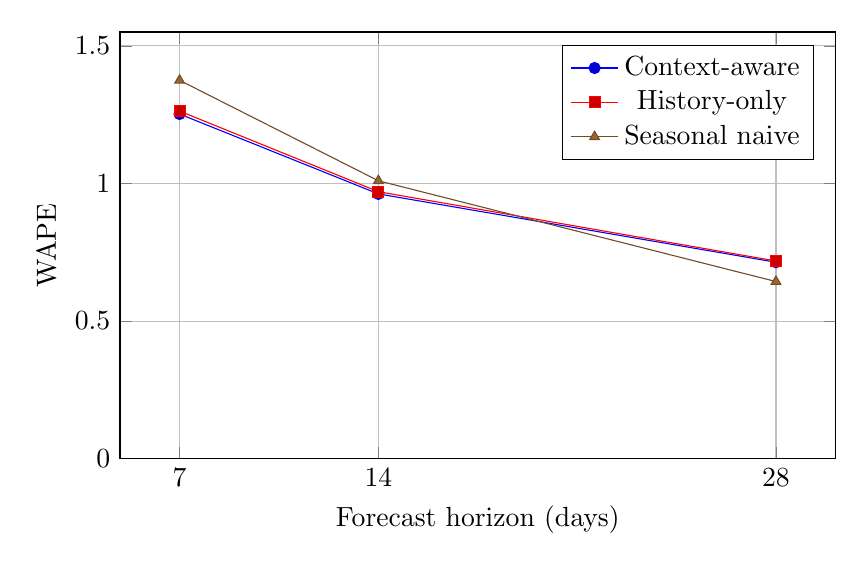
\begin{tikzpicture}
\begin{axis}[width=0.88\textwidth,height=7cm,xlabel={Forecast horizon (days)},ylabel={WAPE},xtick={7,14,28},ymin=0,ymax=1.55,grid=major,legend pos=north east]
\addplot+[mark=*] coordinates {(7,1.2521)(14,0.9620)(28,0.7137)};
\addlegendentry{Context-aware}
\addplot+[mark=square*] coordinates {(7,1.2629)(14,0.9700)(28,0.7182)};
\addlegendentry{History-only}
\addplot+[mark=triangle*] coordinates {(7,1.3746)(14,1.0097)(28,0.6435)};
\addlegendentry{Seasonal naive}
\end{axis}
\end{tikzpicture}
\caption{RQ1 WAPE across forecast horizons. The seasonal-naive baseline is strongest at 28 days.}
\label{fig:rq1_wape}
\end{figure}

\subsection{Higher-Capacity Challenger and Prediction Intervals}
A separate 250-tree LightGBM Tweedie challenger was fitted on the full training partition. It reduces WAPE compared with the 45-tree context model, but MASE remains higher than the seasonal-naive benchmark at every horizon. Its WAPE is 1.220, 0.936 and 0.690 at 7, 14 and 28 days, respectively. The 28-day seasonal-naive WAPE remains lower at 0.644. The challenger is therefore not a universal replacement for the baseline.

The 250-tree model's empirical 80\% residual intervals cover 86.5\%, 86.1\% and 85.5\% of the test observations at 7, 14 and 28 days. Mean interval widths are 2.74, 4.66 and 7.26 units. Coverage is above the nominal 80\%, but intervals widen with the forecast horizon. These intervals are empirical calibration bands, not a guarantee under distribution shift.

\begin{table}[htbp]
\centering
\small
\begin{tabular}{rrrrrr}
\toprule
\textbf{Horizon} & \textbf{Model WAPE} & \textbf{Naive WAPE} & \textbf{Model MASE} & \textbf{Naive MASE} & \textbf{80\% coverage}\\
\midrule
7 days & 1.220 & 1.375 & 0.993 & 0.965 & 86.5\%\\
14 days & 0.936 & 1.010 & 0.790 & 0.738 & 86.1\%\\
28 days & 0.690 & 0.644 & 0.595 & 0.473 & 85.5\%\\
\bottomrule
\end{tabular}
\caption{Exploratory 250-tree context model compared with seasonal naive.}
\label{tab:rq1_challenger}
\end{table}

\section{RQ2: Customer Inactivity Prediction}
The test set contains 21,164 snapshots with a positive outcome rate of 41.18\%. The recency rule improves substantially on the base-rate predictor. LightGBM further improves PR-AUC from 0.687 to 0.731 and Lift@10\% from 1.989 to 2.031. Platt calibration leaves ranking metrics unchanged but improves probability quality: Brier score falls from 0.177 to 0.173 and ECE falls from 0.076 to 0.050.

\begin{table}[htbp]
\centering
\small
\begin{tabular}{lrrrrr}
\toprule
\textbf{Model} & \textbf{PR-AUC} & \textbf{Lift@10\%} & \textbf{Brier} & \textbf{ECE} & \textbf{ROC-AUC}\\
\midrule
Base-rate predictor & 0.412 & -- & 0.247 & 0.069 & 0.500\\
Recency rule & 0.687 & 1.989 & 0.198 & 0.057 & 0.756\\
LightGBM raw & 0.731 & 2.031 & 0.177 & 0.076 & 0.820\\
LightGBM Platt-calibrated & 0.731 & 2.031 & 0.173 & 0.050 & 0.820\\
\bottomrule
\end{tabular}
\caption{RQ2 temporal test results on 21,164 customer snapshots.}
\label{tab:rq2_metrics}
\end{table}

Customer-cluster bootstrap intervals are 0.720--0.743 for PR-AUC, 1.986--2.076 for Lift@10\%, 0.170--0.176 for Brier score and 0.044--0.056 for ECE. The two test cut-offs have PR-AUC values of 0.709 and 0.749, respectively. The model is useful for ranking the supplied temporal test population, but the evaluation is not a cold-start test and does not prove that a marketing intervention will change customer behaviour.

\begin{figure}[htbp]
\centering
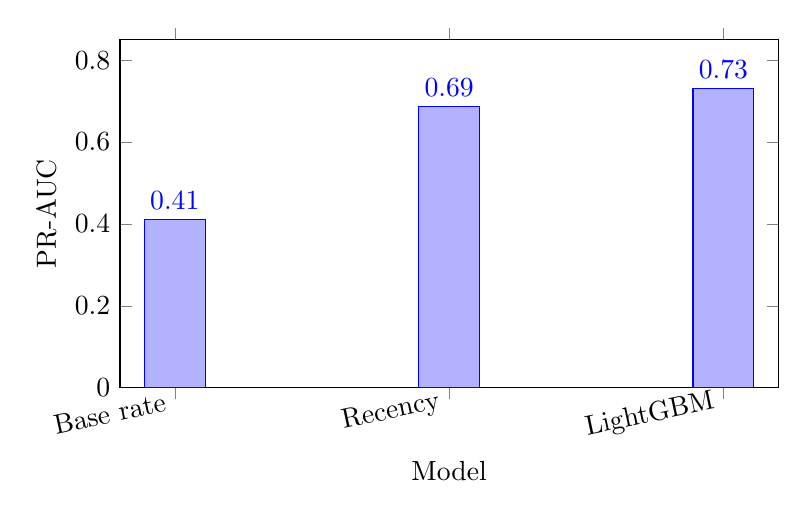
\begin{tikzpicture}
\begin{axis}[ybar,width=0.82\textwidth,height=6cm,symbolic x coords={Base rate,Recency,LightGBM},xtick=data,ymin=0,ymax=0.85,ylabel={PR-AUC},xlabel={Model},nodes near coords,bar width=22pt,x tick label style={rotate=12,anchor=east}]
\addplot coordinates {(Base rate,0.4118)(Recency,0.6874)(LightGBM,0.7315)};
\end{axis}
\end{tikzpicture}
\caption{RQ2 PR-AUC comparison. The calibrated and raw LightGBM models share the same ranking.}
\label{fig:rq2_prauc}
\end{figure}

\section{RQ3: Replenishment Policy Evidence}
The historical procurement ledger contains 122,422 purchase orders and 122,422 purchase lines across 32 shops and 56 suppliers. Of these orders, 113,073 are marked received, 8,034 partial and 1,315 pending at the data cut-off. There are 121,107 orders with an actual delivery date. Observed supplier lead time has a mean of 7.74 days, a median of 7 days and a 90th percentile of 13 days.

The separate scenario file contains 2,500 shop--SKU cases at the 31 July 2025 cut-off. The trend scenario orders 654 units compared with 7,356 units in the supplied baseline. Supplied scenario cost falls by BDT 19,400.60 (0.87\%), from BDT 2,227,690.07 to BDT 2,208,289.47. However, scenario stock-out units rise from 45 to 100, an increase of 55 units or 122.2\%. Mean average stock falls by 1.34\%.

\begin{table}[htbp]
\centering
\small
\begin{tabular}{lrrr}
\toprule
\textbf{Scenario measure} & \textbf{Baseline} & \textbf{Trend policy} & \textbf{Change}\\
\midrule
Order units & 7,356 & 654 & -91.1\%\\
Stock-out units & 45 & 100 & +122.2\%\\
Mean average stock (units) & 157.13 & 155.03 & -1.34\%\\
Total scenario cost (BDT) & 2,227,690.07 & 2,208,289.47 & -0.87\%\\
\bottomrule
\end{tabular}
\caption{RQ3 supplied scenario comparison. These are generated scenario outcomes, not observed owner-policy results.}
\label{tab:rq3_scenario}
\end{table}

A 2,000-replicate shop-cluster bootstrap gives a cost-change interval of -1.01\% to -0.73\% and a stock-out difference interval of 32 to 82 units. The cost-gap arithmetic matches the supplied columns to floating-point tolerance. This does not validate the cost model: separate holding, shortage and ordering cost components are absent. The file also does not identify the baseline as the participating owner's written policy. In the seven days before the scenario cut-off, 109 of the 2,500 matched shop--SKU cases have an observed purchase-order line, totalling 9,858 ordered units. This is descriptive historical context and is not a counterfactual policy test.

\begin{figure}[htbp]
\centering
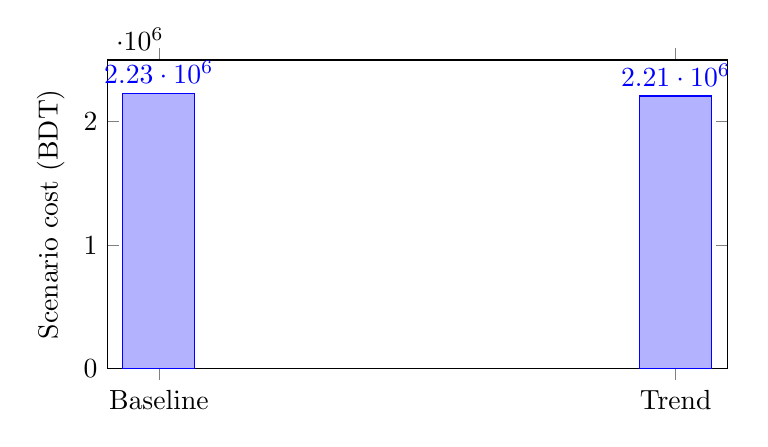
\begin{tikzpicture}
\begin{axis}[ybar,width=0.78\textwidth,height=5.5cm,symbolic x coords={Baseline,Trend},xtick=data,ymin=0,ymax=2500000,ylabel={Scenario cost (BDT)},nodes near coords,bar width=26pt]
\addplot coordinates {(Baseline,2227690.07)(Trend,2208289.47)};
\end{axis}
\end{tikzpicture}
\caption{Supplied RQ3 scenario cost.}
\label{fig:rq3_cost}
\end{figure}

\begin{figure}[htbp]
\centering
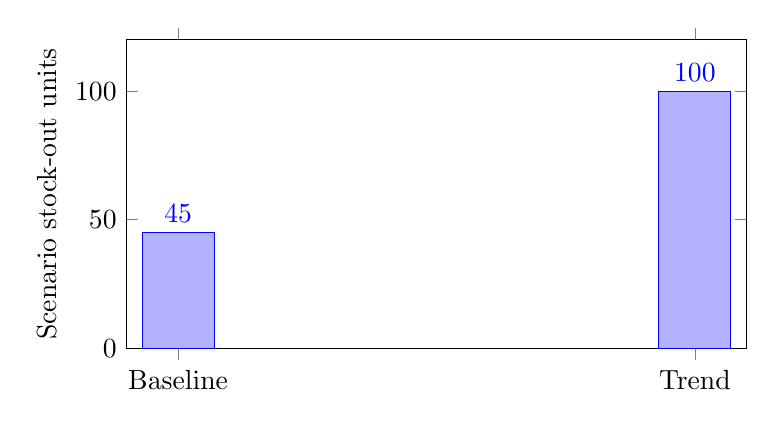
\begin{tikzpicture}
\begin{axis}[ybar,width=0.78\textwidth,height=5.5cm,symbolic x coords={Baseline,Trend},xtick=data,ymin=0,ymax=120,ylabel={Scenario stock-out units},nodes near coords,bar width=26pt]
\addplot coordinates {(Baseline,45)(Trend,100)};
\end{axis}
\end{tikzpicture}
\caption{Supplied RQ3 scenario stock-outs. The lower-cost scenario has more stock-out units.}
\label{fig:rq3_stockout}
\end{figure}

\section{RQ4: Explanation Case Audit}
The RQ4 file contains 1,800 generated cases: 1,601 NO\_ACTION and 199 REORDER. The constraint reasons are 1,600 SUFFICIENT\_STOCK, 199 UNDER\_REORDER\_POINT\_AND\_BUDGET\_OK and one BUDGET\_INSUFFICIENT. All cases have evidence\_complete=YES. The action--quantity rule passes for all 1,800 cases, giving 100\% internal consistency.

This is not a human decision evaluation. The human\_rating column contains YES for every row and no participant or rating scale fields are present. All 1,800 explanation strings refer to synthetic stock wording. The task-preparation step produced 899 matched pairs, two counterbalanced forms with 1,798 tasks each and two reserve cases. No decision correctness, completion time, confidence or usability result can be calculated until consenting users complete the tasks.

\begin{figure}[htbp]
\centering
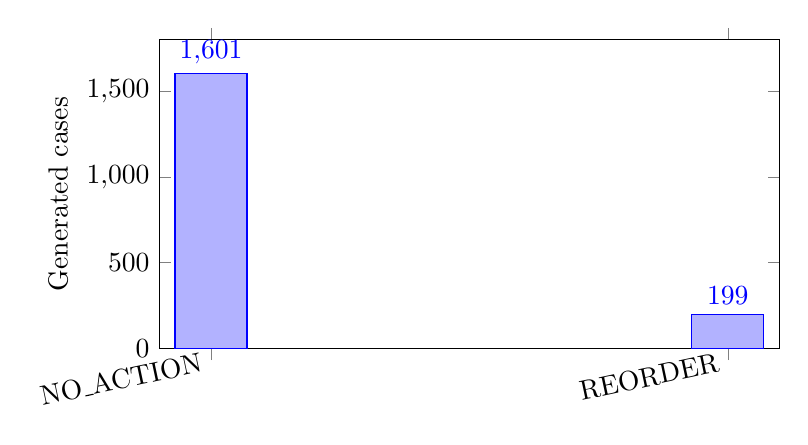
\begin{tikzpicture}
\begin{axis}[ybar,width=0.78\textwidth,height=5.5cm,symbolic x coords={NO\_ACTION,REORDER},xtick=data,ymin=0,ymax=1800,ylabel={Generated cases},nodes near coords,bar width=26pt,x tick label style={rotate=12,anchor=east}]
\addplot coordinates {(NO\_ACTION,1601)(REORDER,199)};
\end{axis}
\end{tikzpicture}
\caption{RQ4 generated action distribution. This figure does not represent user responses.}
\label{fig:rq4_actions}
\end{figure}

\section{Overall Research Question Status}
\begin{table}[htbp]
\centering
\small
\begin{tabularx}{\textwidth}{p{0.7cm} X X}
\toprule
\textbf{RQ} & \textbf{Evidence completed} & \textbf{Remaining evidence}\\
\midrule
RQ1 & Out-of-time branch--SKU experiments, ablations, baselines, interval coverage and bootstrap comparison. & Improve SKU-level accuracy; test on a later untouched period and additional businesses.\\
RQ2 & Temporal LightGBM experiment, recency baseline, Platt calibration and customer-cluster intervals. & Test cold-start customers and evaluate a real intervention before claiming business impact.\\
RQ3 & Historical PO and lead-time audit; supplied scenario comparison and shop-cluster intervals. & Obtain the participating owner's documented policy and validated cost components for a matched replay.\\
RQ4 & Generated-case consistency audit, matched task bank, scoring key and study protocol. & Obtain ethics approval where required and collect outcomes from consenting target users.\\
\bottomrule
\end{tabularx}
\caption{Evidence status against the four research questions.}
\label{tab:rq_status}
\end{table}

\section{Results Analysis}
RQ1 shows that adding context gives a modest WAPE gain over the history-only model, but the gain is not consistent across metrics. MASE favours the seasonal-naive baseline, and the 28-day WAPE also favours that baseline. The current forecasting model should therefore be treated as a research candidate, not as a proven replacement for a simple forecast.

RQ2 provides the strongest completed predictive result. The calibrated LightGBM model ranks future inactive customers better than the recency rule and produces improved probability calibration. The result supports prioritisation on the supplied temporal test set, but it does not show that contacting those customers will prevent inactivity.

RQ3 shows a cost--service trade-off in the supplied scenario. A lower scenario cost is accompanied by more stock-out units. Historical purchase records provide actual lead-time evidence, but the current files do not establish the participating owner's formal replenishment rule or the cost components needed for a validated policy comparison.

RQ4 confirms that the generated action and quantity fields agree with the rule encoded in the case file. That is an internal consistency check only. User comprehension, decision quality and perceived usability remain unmeasured.

\section{Limitations}
The dataset covers one retail business type, and source provenance is declared by the project owner but not independently audited in this report. RQ1 has only three monthly test origins and high per-series error. RQ2 is not a cold-start evaluation. RQ3 relies on a single-cut-off generated demand scenario and supplied cost columns without decomposed assumptions. RQ4 has no participant observations. These limitations constrain the conclusions and must be addressed before the system is presented as fully validated.
